%!TEX root = ../TAMUTemplate.tex
%%%%%%%%%%%%%%%%%%%%%%%%%%%%%%%%%%%%%%%%%%%%%%%%%%%
%
%  New template code for TAMU Theses and Dissertations starting Fall 2016.
%
%  Author: Sean Zachary Roberson
%	 Version 3.16.09
%  Last updated 9/12/2016
%
%%%%%%%%%%%%%%%%%%%%%%%%%%%%%%%%%%%%%%%%%%%%%%%%%%%

%%%%%%%%%%%%%%%%%%%%%%%%%%%%%%%%%%%%%%%%%%%%%%%%%%%%%%%%%%%%%%%%%%%%%%%
%%%                           SECTION II
%%%%%%%%%%%%%%%%%%%%%%%%%%%%%%%%%%%%%%%%%%%%%%%%%%%%%%%%%%%%%%%%%%%%%%


\chapter{\uppercase {The LHC and CMS Detector}}
\label{ch:LHC_CMS}

\section{The Large Hadron Collider}
\label{sec:LHC}

The Large Hadron Collider (LHC) \cite{Breskin:1244506} is, in many people's estimation, the largest and most complex machine ever built by humanity.
The main accelerator at the European Organization for Nuclear Research (CERN), the LHC is located both in France and Switzerland due to its enormous size (Fig.~\ref{fig:LHC_schematic}).
It was built between 1998 and 2008 and installed in the 26.7\unit{km} tunnel dug for its predecessor, the Large Electron-Positron Collider (LEP), which is located between 50\unit{m} and 170\unit{m} underground.
It is the highest energy collider in the world, eclipsing the previous record holder, the Tevatron at Fermilab in Batavia, IL.
The following section is a description of the LHC and CERN accelerator complex based on \cite{LHCmachine} and \cite{Breskin:1244506}.

\begin{figure}[!hbt]
	\vspace*{-0.5cm}
	\centering
	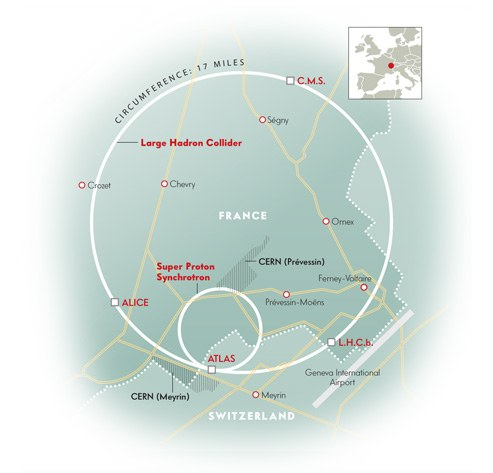
\includegraphics[width=0.95\textwidth]{\figpath/Chapter2/LHC_schematic.jpg}
	\caption{Overhead view of CERN and its main experiments, CMS; ATLAS; LHCb; and ALICE, as well as two of the larger accelerators, the LHC and SPS. The schematic is overlaid on a map of Switzerland and France~\cite{LHC-schematic}.}
	\label{fig:LHC_schematic}
\end{figure}

The LHC provides beams for four main experiments located along its beam line (Fig.~\ref{fig:LHC_schematic}):
\begin{itemize}
	\item The CMS (Compact Muon Solenoid)~\cite{Chatrchyan:2008aa} and ATLAS (A Toroidal LHC ApparatuS)~\cite{1748-0221-3-08-S08003} experiments are both general purpose detectors. Their goals include precision measurements to test the Standard Model and searches for new physics, including the Higgs boson.
	\item LHCb (Large Hadron Collider beauty)~\cite{Alves:2008zz} was designed to do precision measurements of CP-violation and the physics of B-mesons.
	\item ALICE (A Large Ion Collider Experiment)~\cite{Aamodt:2008zz} studies heavy ion collisions.
\end{itemize}

The LHC was designed to collide two beams of protons (pp), heavy ions (PbPb), or a combination of the two (pPb) at specific interaction points around the beam line.
For the purposes of this thesis we will only cover proton-proton collisions from this point forward.
The protons come from a single bottle of hydrogen gas, which is then disassociated and stripped of electrons to form a proton beam.
Interestingly, only 1\unit{ng} of hydrogen is required per day in order to form the LHC beams.
The protons next travel through the Linac2 machine where they are bunched by radio frequency (RF) electromagnetic fields and are accelerated to 50\MeV.
This chain continues through the Proton Synchroton Booster (PSB), the Proton Synchrotron (PS), and the Super Proton Synchrotron (SPS) where the protons are accelerated to 1.4\GeV, 26\GeV, and 450\GeV respectively (Fig.~\ref{fig:CERN_accelerators}).

\begin{sidewaysfigure}[!hbt]
	\centering
	\begin{subfigure}[t]{0.4655\textwidth}
		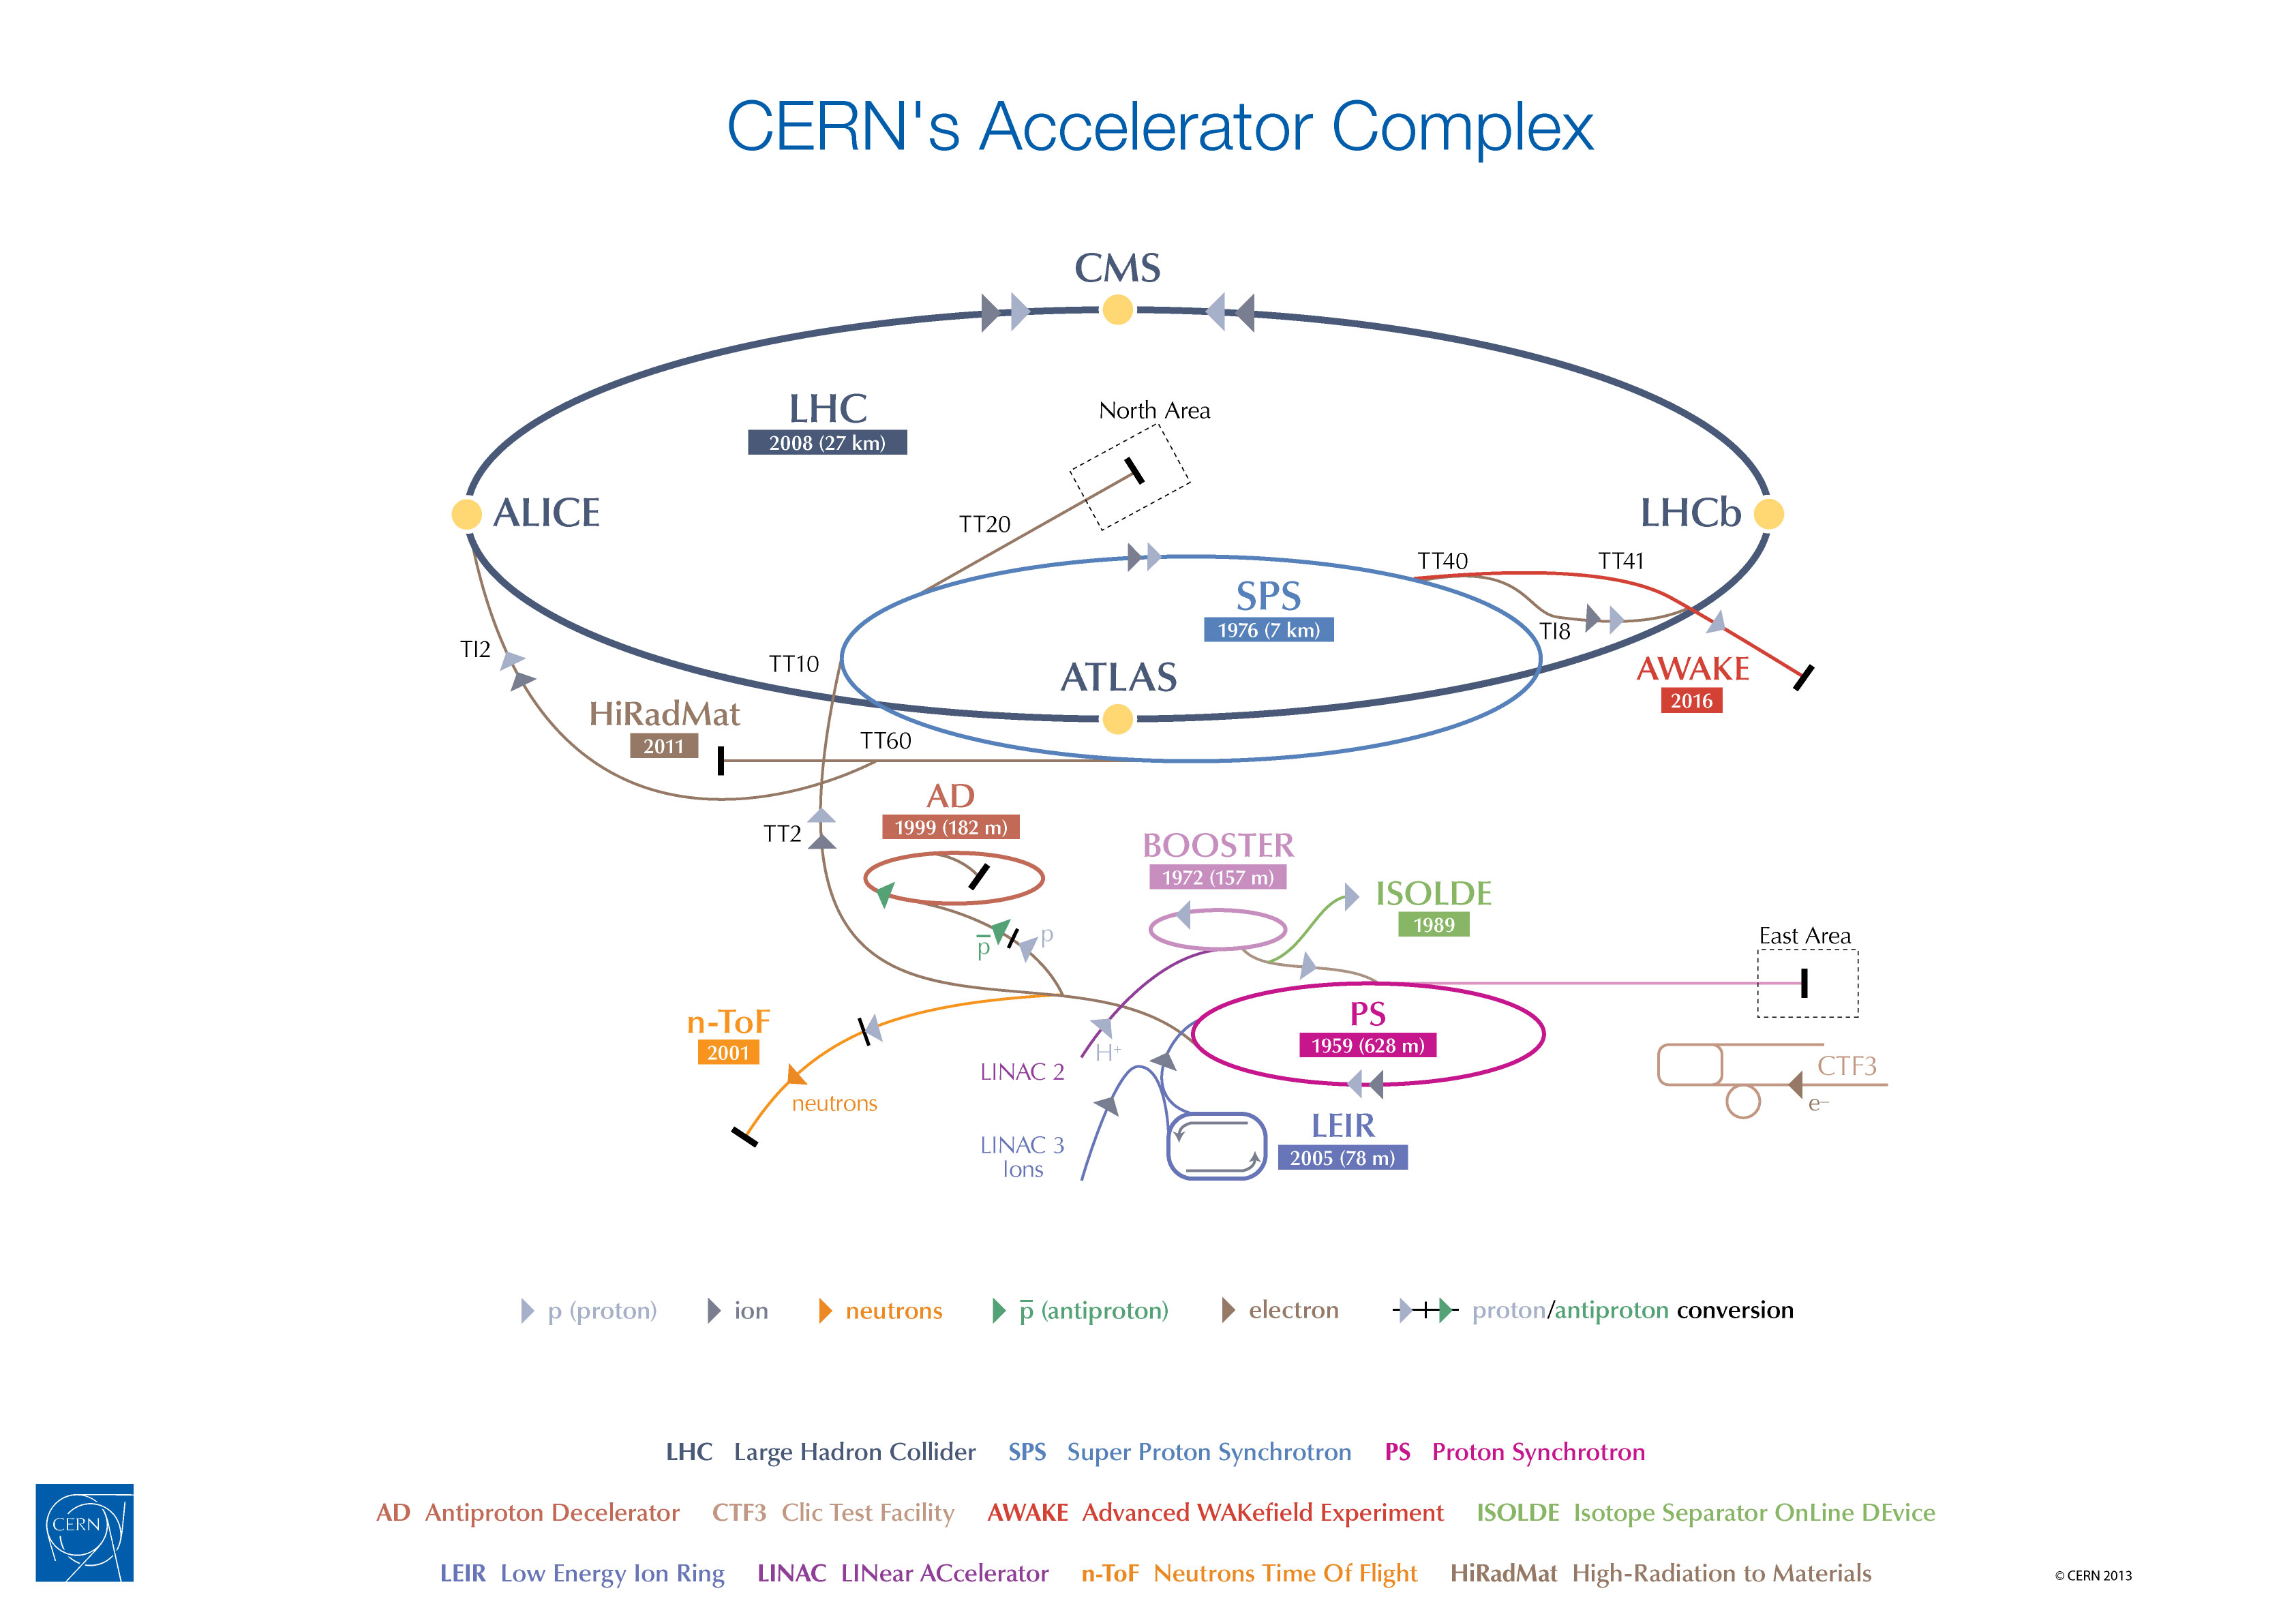
\includegraphics[width=\textwidth]{\figpath/Chapter2/CERN's-accelerator-complex2013.jpg}
		\label{fig:CERN_accelerator_complex}
	\end{subfigure}
	\begin{subfigure}[t]{0.4655\textwidth}
		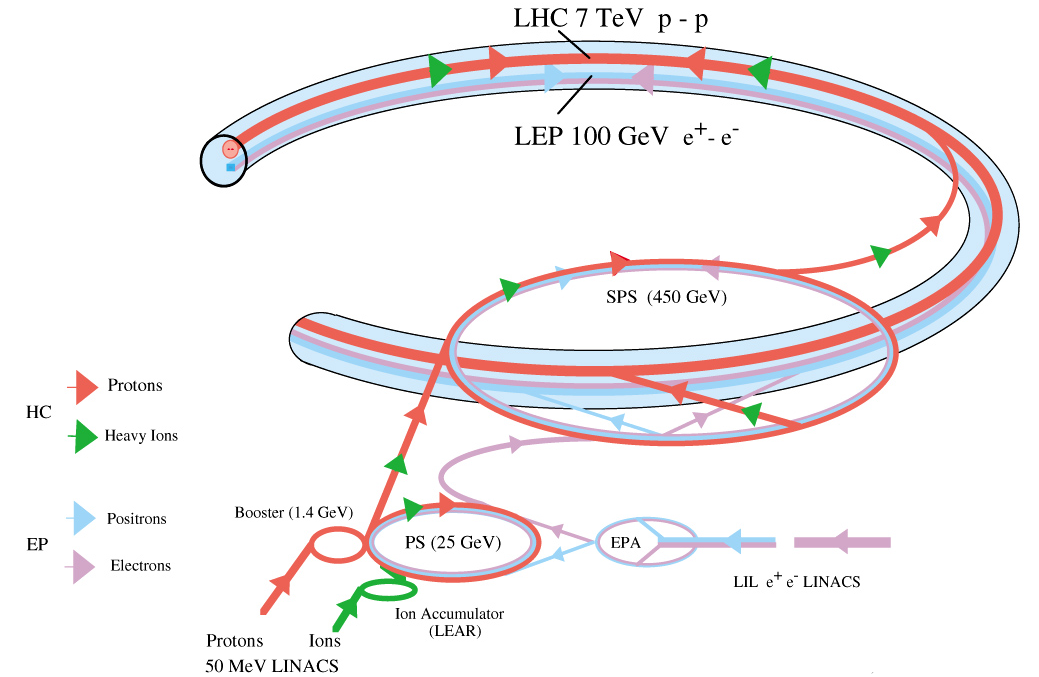
\includegraphics[width=\textwidth]{\figpath/Chapter2/lhc-pho-1993-008.png}
		\label{fig:LHC_LEP_injection_complex}
	\end{subfigure}
	\caption{Left: A schematic of the CERN accelerator complex~\cite{Marcastel:1621583}. Right: A diagram of the LHC injection chain. Also included is a diagram of the heavy ion and LEP injection chains~\cite{Jean-Luc:841568}.}
	\label{fig:CERN_accelerators}
\end{sidewaysfigure}

\clearpage

After being accelerated in the SPS, the proton bunches are injected into the two LHC beam pipes, which were designed to accelerate the two proton beams to 7\TeV (Fig~\ref{fig:LHC_beams}).
Size limitations in the tunnel dictated that the the beam lines be formed by twin bore magnets.
Each magnet is formed by a single mechanical structure and cryostat while containing two coils and two beam channels.
The coils are made out of superconducting NbTi Rutherford cables cooled to 1.9\unit{K} by 120\unit{t} of superfluid helium.
This forms the 8.33\unit{T} magnets necessary for bending the 7\TeV protons (Fig.~\ref{fig:LHC_magnet}).
The LHC contains 1232 superconducting dipole magnets for bending the protons and 392 superconducting quadrupole magnets for focusing the beams.
The beam line also contains sextapole, octopole, and decapole magnets, which are also used to correct and focus beams.
The original LHC design calls for a bunch spacing of 25\unit{ns}, $10^{11}$ protons per bunch, and 2808 bunches per beam.
%The acceleration is accomplished by 16 RF cavities operating at 400MHz.

\begin{figure}[!hbt]
	\centering
	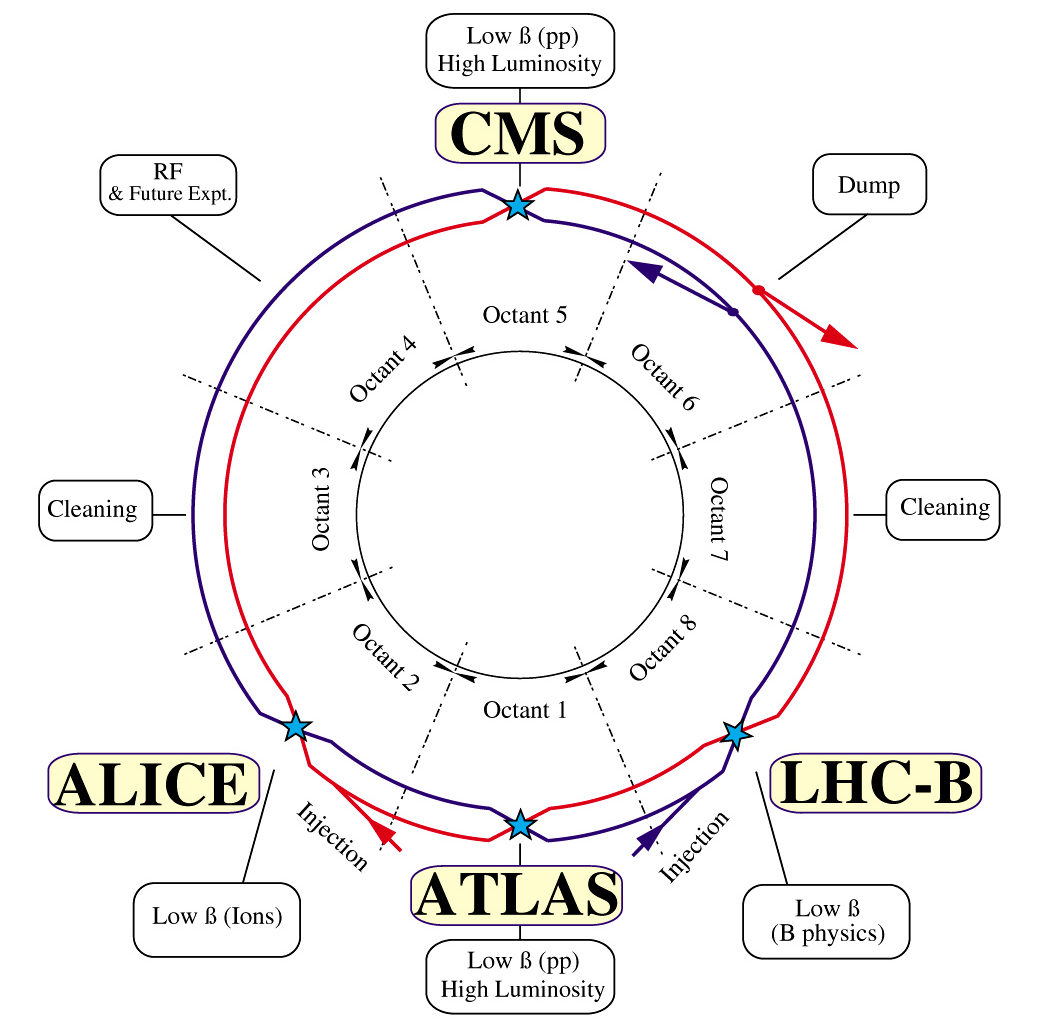
\includegraphics[width=0.95\textwidth]{\figpath/Chapter2/lhc-pho-1997-060.png}
	\caption{A diagram of the LHC beams along with the four major experiments~\cite{Jean-Luc:841573}.}
	\label{fig:LHC_beams}
\end{figure}

\begin{figure}[!hbt]
	\centering
	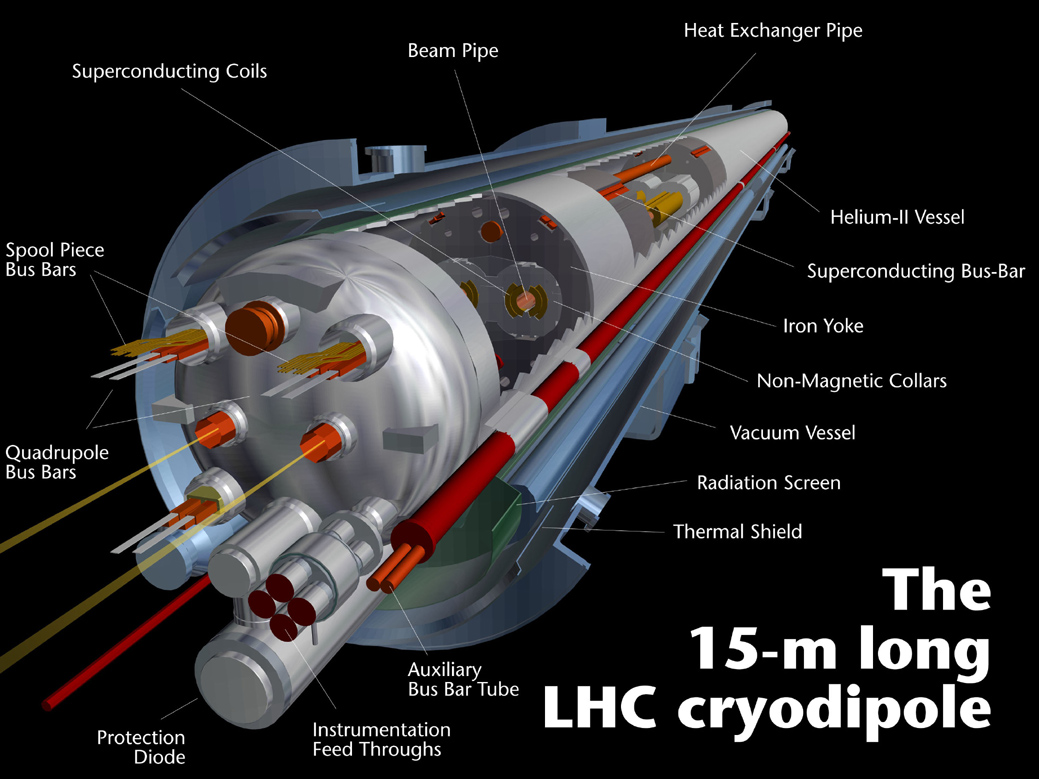
\includegraphics[width=0.95\textwidth]{\figpath/Chapter2/lhc-pho-1998-299.jpg}
	\caption{A diagram of an LHC dipole magnet and cryostat~\cite{Dailler:842253}.}
	\label{fig:LHC_magnet}
\end{figure}

The original plan was to start the LHC accelerator complex in September 2008.
However, due to a catastrophic incident damaging the machine, the startup was delayed until November 23, 2009; even then colliding beams only had a center-of-mass energy of 900\GeV.
From March 30, 2010 through the end of 2011 the LHC operated with a center-of-mass energy of 7\TeV.
Then in 2012 the energy was again increased to 8\TeV (4\TeV per beam), which is the energy of the beams during the data-taking period focused on by this thesis.
It is important to note, though, that the machine has continued to operate after the 2012 data taking period and increased the center-of-mass energy to 13\TeV starting in 2015 (there was a planned shutdown from 2013 through early 2015).

In addition to the center-of-mass energy, collider physicists are interested in the rate at which a specific physics process occurs.
This in turn is related to the cross sections, the probability that two particles will collide and react a certain way, and the luminosity.
The rate of events is given by equation~\ref{eq:dn/dt}, where $\mathcal{L}$ is the collision luminosity and $\sigma$ is the cross section for a given physical process.

\begin{equation}
dN/dt=\mathcal{L}{\cdot}\sigma
\label{eq:dn/dt}
\end{equation}

The luminosity as it is described here is often called the ``instantaneous luminosity'' as this value can change from moment to moment.
The ``integrated luminosity'' is then a measure of the total amount of data collected.
The instantaneous luminosity itself depends upon the parameters of the LHC beams and the optical properties of the focusing system at the interaction point.
This information is summed up in equation~\ref{eq:luminosity}~\cite{1742-6596-455-1-012001}:

\begin{equation}
\mathcal{L}=\frac{N^{2}n_{b}f\gamma}{4\pi\epsilon_{n}\beta^{*}}F
\label{eq:luminosity}
\end{equation}

where:

\begin{itemize}
	\item $N$: protons per bunch
	\item $n_{b}$: bunches in the LHC ring
	\item $f$: frequency of bunch revolutions around the ring 
	\item $\gamma$: relativistic factor for the protons
	\item $\epsilon_{n}$: normalized emittance of the proton beams
	\item $\beta^{*}$: beta function at the interaction point
	\item $F$: geometrical reduction factor due to the crossing angle of the beams
\end{itemize}

The maximum design luminosity of the LHC is $1\times10^{34}\percms$.
During the 2010 and 2011 run periods (7\TeV center-of-mass energy) the instantaneous luminosity increased from $1\times10^{32}\percms$ to $5\times10^{33}\percms$.
During the 2012 data-taking period, the peak instantaneous luminosity was $7.67\times10^{33}\percms$ with a bunch spacing of 50\unit{ns}, a maximum number of bunches of 1380, and $\sim2.2\times10^{14}$ protons per beam ($\sim1.6\times10^{11}$ protons per bunch).
The LHC delivered 23.30\fbinv of integrated luminosity to the CMS detector of which 21.79\fbinv was recorded.
As of the end of 2016, the LHC is still running at 13\TeV (6.5\TeV per beam) with a peak luminosity of $1.53\times10^{34}\percms$, 2208 bunches, and $1\times10^{11}$ protons per bunch~\cite{CMSWebBasedMonitoring,LumiPublic}.
Figures~\ref{fig:LHC_int_lumi_pp} and~\ref{fig:LHC_lumi_per_day_pp} show the total integrated luminosity delivered by the LHC and recorded by the CMS experiment for the various data-taking periods~\cite{LumiPublic}.

\begin{figure}[!hbt]
	\centering
	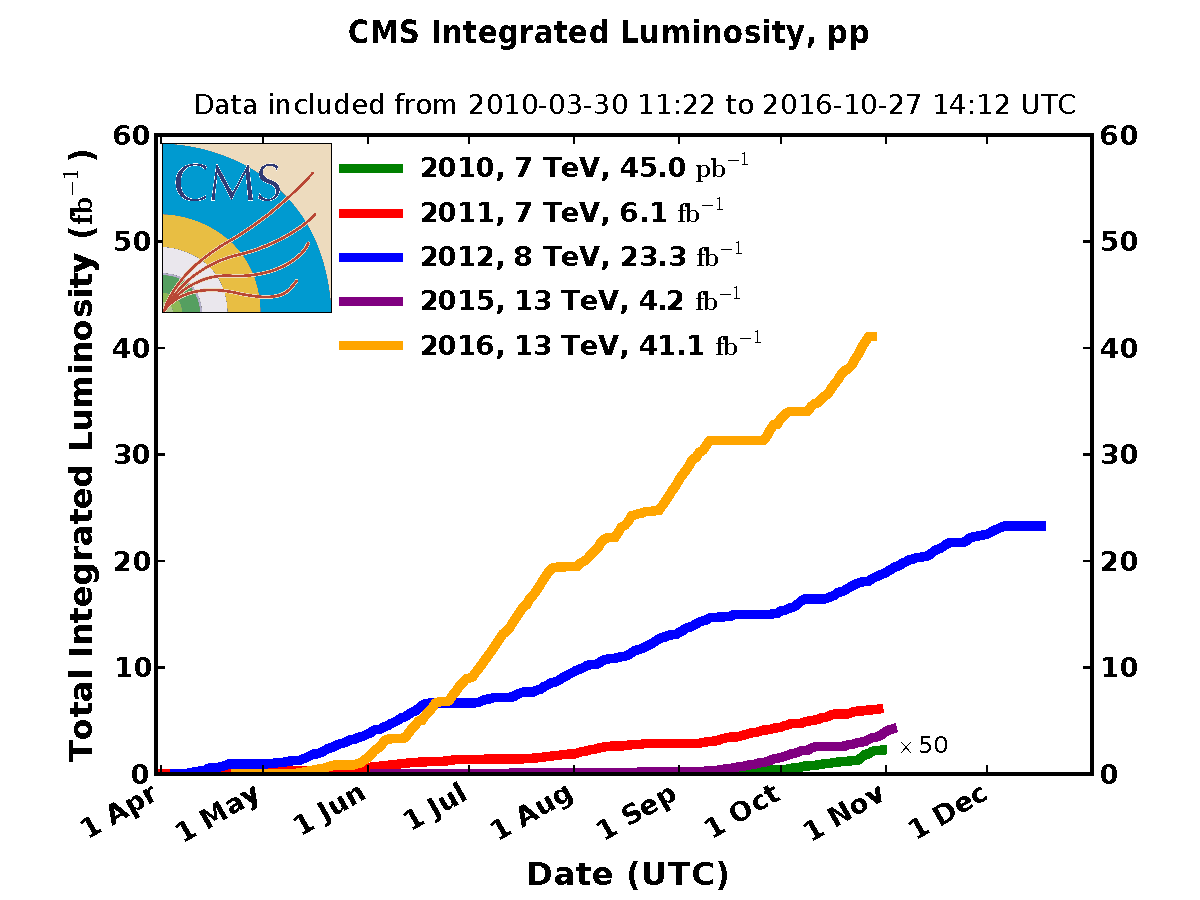
\includegraphics[width=0.95\textwidth]{\figpath/Chapter2/int_lumi_cumulative_pp_2.pdf}
	\caption{Total integrated luminosity versus time delivered to the CMS experiment for the 2010, 2011, 2012, 2015, and 2016 p-p data-taking periods~\cite{LumiPublic}.}
	\label{fig:LHC_int_lumi_pp}
\end{figure}

\begin{figure}[!hbt]
	\centering
	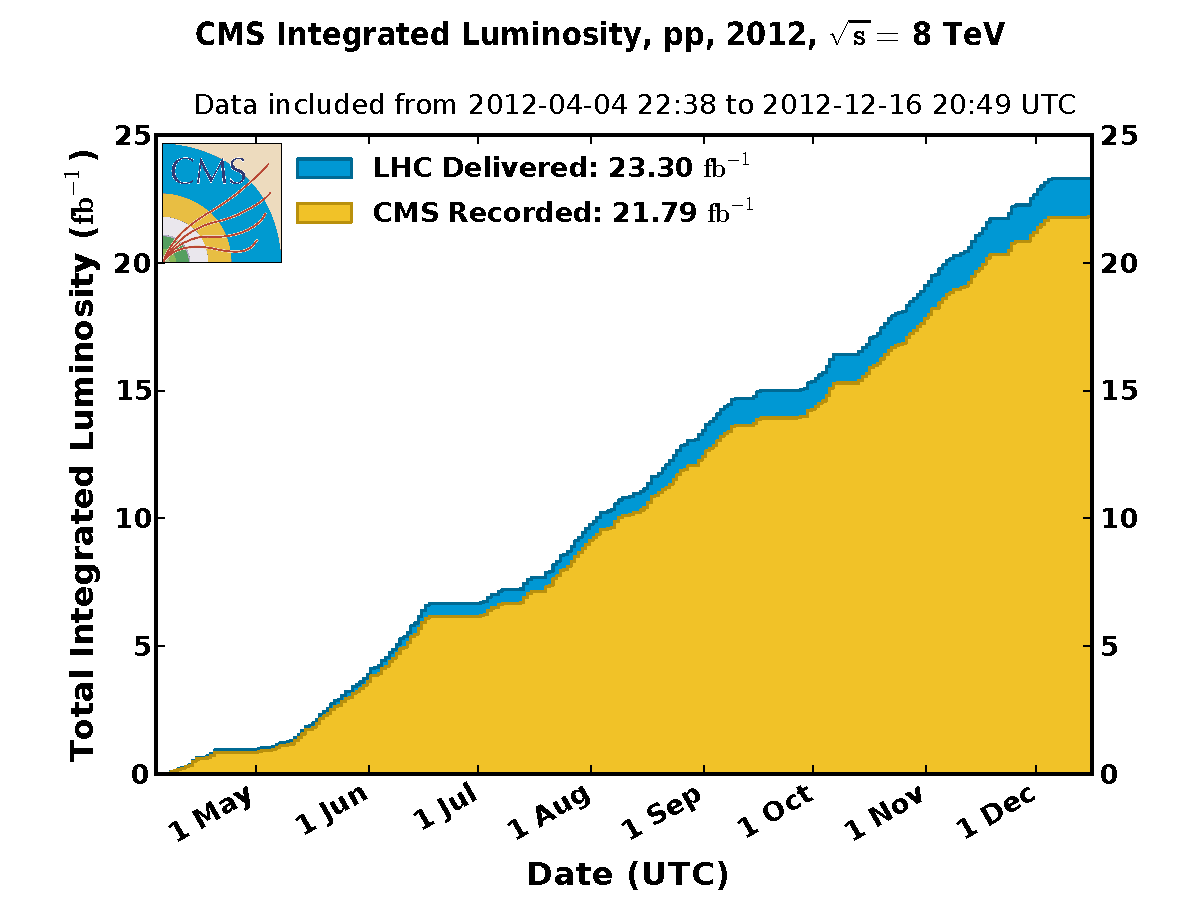
\includegraphics[width=0.95\textwidth]{\figpath/Chapter2/int_lumi_per_day_cumulative_pp_2012.pdf}
	\caption{Total integrated, offline luminosity versus day in 2012. The blue graph shows the delivered luminosity while the orange graph shows the luminosity recorded by the CMS experiment. This graph shows only the luminosity collected for p-p collisions during stable beams~\cite{LumiPublic}.}
	\label{fig:LHC_lumi_per_day_pp}
\end{figure}


\section{The CMS Detector}

TALK ABOUT THE PHYSICS GOALS?
%"The physics program of the experiment covers a wide range of goals: precision study of Standard Model processes, study of properties of the recently discovered Higgs boson, searches for physics beyond the Standard Model, and study of quark-gluon plasma." - Aysen Tatarinov

The CMS experiment is one of two general purpose detectors at the LHC; ATLAS being the other one.
The detector is located 100\unit{m} underground near Cessy, France on the opposite side of the LHC from the main CERN site in Meyrin (see figure~\ref{fig:LHC_schematic}).
It was largely built on the surface and then lowered into the collision cavern in 15 pieces, which then had to be painstakingly assembled.
The detector has a cylindrical design which is 22\unit{m} in length, 15\unit{m} in diameter, and weights 14000 tonnes.
The shape and positioning of the detector around the interaction point (IP) gives the experiment nearly $4\pi$ coverage of the proton-proton collisions.
The layout of the detector can be seen in fig.~\ref{fig:CMS_schematic}.

Fig.~\ref{fig:CMS_transverse} shows how various types of particles interact within the CMS sub-detectors.
In total, there are ${\sim}10^8$ data channels checked in each bunch crossing owing to the high granularity of the CMS sub-detectors.
The following sections will describe each of the sub-detectors and its properties and is based largely on Ref.~\cite{Chatrchyan:2008aa}.

\begin{figure}[!hbt]
	\centering
	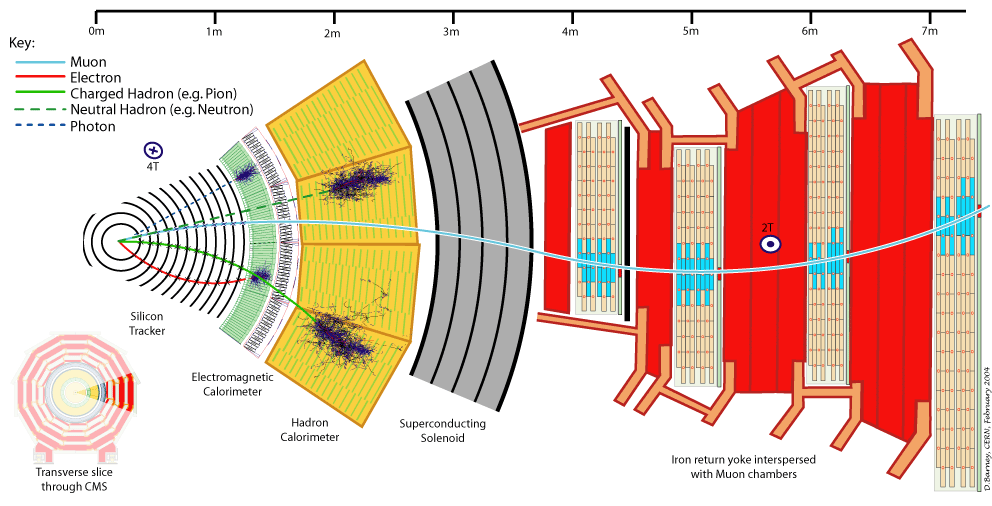
\includegraphics[width=0.95\textwidth]{\figpath/Chapter2/CMS_slice.png}
	\caption{Transverse slice of the CMS experiment with the major sub-detectors and components represented. The different colored lines represent how various types of particles interact with the sub-detectors~\cite{CMSSlice}.}
	\label{fig:CMS_transverse}
\end{figure}

\subsection{Coordinate System}

The IP is at the center of the detector and is the origin of the right-handed coordinate system used to describe the detector and the physics being measured (location and direction).
The $z$-axis is defined along the LHC beam line.
Instead of using the polar angle, $\theta$, which would go from $0^{\degree}$ along the positive $z$-axis to $90^{\degree}$ pointing straight up from the interaction point, collider physicists use the quantity pseudorapidity defined as $\eta=-ln\left[\tan\left(\theta/2\right)\right]$.
The benefits of using the pseudorapidity are that differences in this coordinate, $\Delta\eta$, are invariant under boosts in the $z$-direction and particle production is roughly uniform in $\eta$.
The $x$- and $y$-axes form the plane perpendicular to the $z$-axis, where positive $x$ points to the center of the LHC ring and positive $y$ points upward.
The azimuthal angle, $\varphi$, and radial coordinate, $r$, are also defined in this same plane.
It is sometimes more useful to use $\varphi$ and $r$ due to the bending of the particles in the magnetic field.
Lastly, this paper will often refer to the quantity \pt, which is the magnitude of the component of the momentum vector in the transverse plane.
A schematic of the coordinate system described above is shown in fig.~\ref{fig:CMS_coordinate_system}.

\begin{figure}[!hbt]
	\centering
	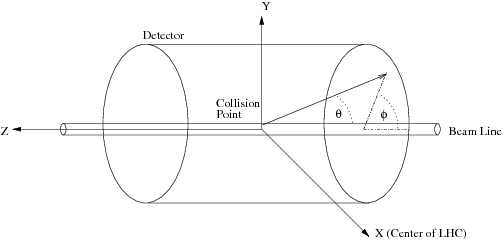
\includegraphics[width=0.95\textwidth]{\figpath/Chapter2/Figures_T_Coordinate.png}
	\caption{Schematic of the CMS coordinate system~\cite{Schott:2014sea}.}
	\label{fig:CMS_coordinate_system}
\end{figure}

\subsection{Tracker and Pixel Detector}
\label{sec:tracker_and_pixel}

The CMS all-silicon tracker is the closest sub-detector to the LHC beam pipe.
Its purpose is twofold; to determine the charged-particle direction at its production vertex and to measure the momentum of charged particles.
In the later case, the tracker is far superior to the calorimeter systems for \pt up to several hundred \gev.
The sub-detector is 5.8\unit{m} long and 2.5\unit{m} in diameter, covering a pseudorapidity range of $\abs{\eta}<2.5$.
It is, by necessity, highly granular, to keep the occupancy low, and relatively radiation hard.
The tracker is exposed to extreme doses of radiation ranging from 0.18 to 84\unit{Mrad} after 500\fbinv of data.
The radiation tolerance was a key factor in determining the materials and design of the sensors and on-board electronics of the tracker.
To keep the radiation damage as low as possible, among other benefits, the tracker is kept at $-10\degC$.
For non-isolated particles of $1<\pt<10\GeV$ and $\abs{\eta}<1.4$, the track resolutions are typically 1.5\% in \pt and 25--90 (45--150)\mum in the transverse (longitudinal) impact parameter.
On the other hand, isolated particles of $\pt=100\GeV$ emitted at $\abs{\eta}<1.4$ have track resolutions of 2.8\% in \pt and 10 (30)\mum in the transverse (longitudinal) impact parameter~\cite{TRK-11-001}.
At higher $\eta$ the reduced transverse depth of the tracker degrades the resolution (particles traverse fewer layers).
Fig.~\ref{fig:CMS_tracker} shows the layout of the tracker and its subsystems. The tracker is formed by two major subsystems, the pixel detector and the silicon strip tracker.


\begin{figure}[!hbt]
	\centering
	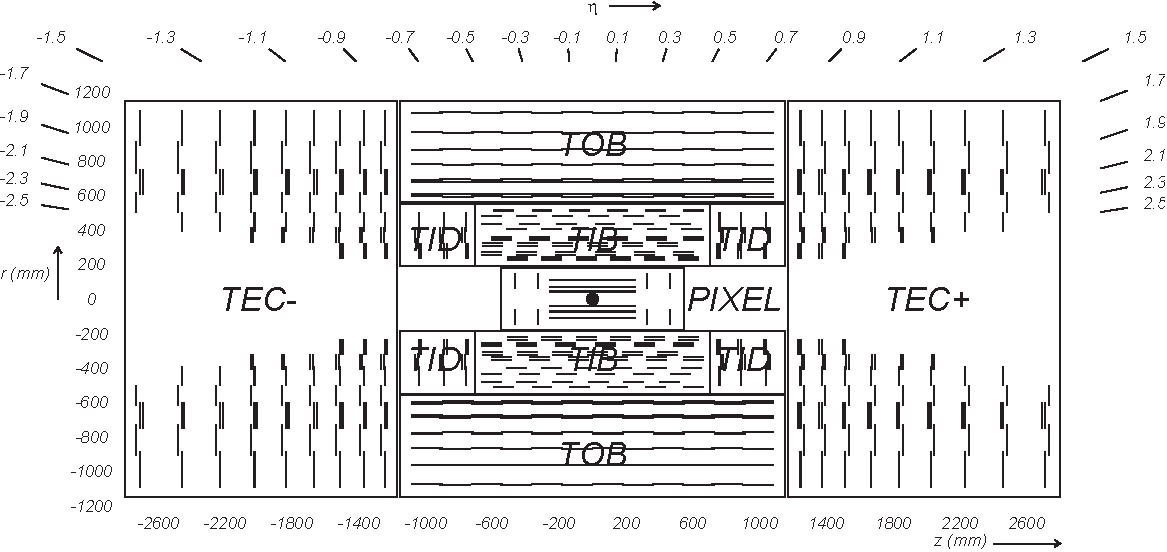
\includegraphics[width=0.95\textwidth]{\figpath/Chapter2/CMS_tracker.pdf}
	\caption{Layout of the CMS tracker with subsystems labeled.}
	\label{fig:CMS_tracker}
\end{figure}

The pixel detector is made up of three barrel layers, called the BPIX, and two endcap layers called the FPIX.
The BPIX contains 48 million pixels and the FPIX contains another 18 million pixels.
In total it consists of 1440 hybrid silicon detector modules, each with a dimension of $100\times150\mum^{2}$.
The small pixel size enables track resolutions of 10\mum in the transverse plane and 20\mum in the $z$-direction.
The pixel detector is what gives CMS its excellent secondary vertex tagging ability in addition to producing seed tracks for the strip tracker and the high level trigger.
NOT SURE I LIKE THIS LAST SENTENCE

Just as the pixel detector was made up of the BPIX and FPIX subsystems, the silicon strip detector is made up of four subsystems.
The Tracker Inner Barrel
(TIB) has four layers of 320\mum strips.
At each end of the TIB is a three-layer Tracker Inner Disks (TID), which contains strips of the same thickness.
The Tracker Outer Barrel (TOB) is the six layer system which surrounds the TIB/TID.
The first four layers of the TOB use 500\mum thick strips, and the last two layers use 122\mum thick strips.
The Tracker EndCaps (TEC) are on either side of the previous setup and contains nine disks with up to seven layers of strips.
These strips are 320\mum thick in the inner four rings and 500\mum thick in the outer three rings.
In total, the strip detector contains 9.3 million silicon strips (15\,148 modules).

The 2012 LHC run was an excellent year for the tracker.
The BPIX maintained 97.7\% of its channels operational while the FPIX had 92.8\% of its channels operational.
The reconstruction efficiencies were also quite high, 99.5\%, for each later of the pixel detector ($>$99.2\% for the first layer).
The strip detector maintained 97.5\% of its channels active and had a reconstruction efficiency greater than 99\% for each layer\cite{Veszpremi:2014hpa}. 

\subsection{Electromagnetic Calorimeter}

The electromagnetic calorimeter (ECAL) is a homogeneous detector consisting entirely of 75\,848 lead tungstate crystals (\PbWO).
The detector is divided up into two sections which provide coverage in pseudorapidity \absetalt{1.479} in a barrel region (EB) and \abseta{1.479}{3.0} in two endcap regions (EE).
There are also preshower detectors (PS) in each of the endcaps, in front of the EE, which cover a pseudorapidity range of \abseta{1.653}{2.6}.
Fig.~\ref{fig:CMS_ECAL} shows the structure of the detector with the key $\eta$ values labeled.

\begin{figure}[!hbt]
	\centering
	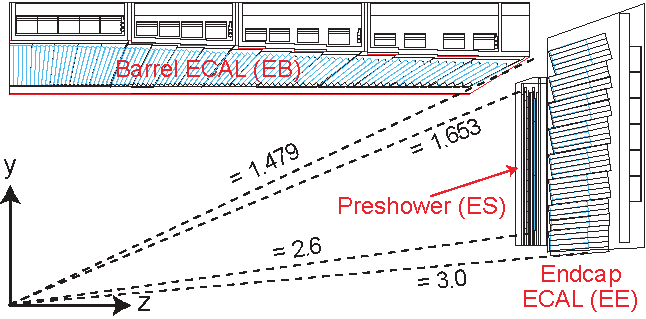
\includegraphics[width=0.95\textwidth]{\figpath/Chapter2/ECAL_transverse_section.pdf}
	\caption{A schematic of the CMS ECAL detect with labeled subsystems and key $\eta$ ranges marked.}
	\label{fig:CMS_ECAL}
\end{figure}

The barrel region of the ECAL consists of 61\,200 crystals with a tapered shape arranged in a projective geometry. Each crystal is about \mytimes{0.0174}{0.0174} in $\eta-\varphi$, which corresponds to \mytimes{22}{22}\unit{mm$^{\text{2}}$} at the front face and \mytimes{26}{26}\unit{mm$^{\text{2}}$} at the back face. Each crystal has a depth of 230\mm, which for \PbWO corresponds to 25.8 radiation lengths ($X_{0}$). The scintillation light produced in the crystals is read out by avalanche photodiodes (APDs), which produce approximately 4.5 photoelectrons per \MeVns at 18\degC. The dark current of the APDs is sensitive to radiation exposure. During the 2012 run, the dark current ranged from 0.13 to 1.3\muA on average, which corresponds to an average noise of 47 to 57\mev~\cite{CMS:2013ecal}.

The EE contains 14\,648 \PbWO crystals arranged in a non-projective $x-y$ geometry (see fig.~\ref{fig:CMS_ECAL}). The crystal dimensions are \mytimes{28.62}{28.62}\unit{mm$^{\text{2}}$} at the front face and \mytimes{30}{30}\unit{mm$^{\text{2}}$} at the back face with a depth of 220\mm or 24.7 $X_{0}$. Instead of using APDs link in the EB, the EE uses vacuum phototriodes (VPTs) to read out the scintillation light. Again holding the photodetectors at 18\degC, the phototriodes produce 4.5 photoelectrons per \MeVns. The average noise in the VPTs for 2012 was 180--200\mev, but it could reach 600\mev at high $\eta$ due to the higher radiation doses in the more forward regions~\cite{CMS:2013ecal}.

The ES is located in front of each of the EE detectors. It consists of two planes of silicon strip sensors interleaved with a total of $3 X_0$ of lead absorber (2 $X_{0}$ for the first layer and 1 $X_{0}$ for the second layer). The silicon strips are 320\mum thick and can collect 3.6\unit{fC} of charge from a minimum ionizing particle (MIP).

One of the main goals of the CMS experiment was to discover the Higgs boson.
Because of its low irreducible standard model background, the $H\rightarrow\gamma\gamma$ channel was considered the ``golden channel''.
Due to this, a significant amount of money and time was spent on the design and the materials for the ECAL.
\PbWO is a great choice for an ECAL because its properties, listed in table~\ref{tab:PbWO4Properties}, lead to a precision energy measurement for EM objects (by this I mean a fine small resolution). 

\DTLnewdb{PbWO4Data}
\DTLnewrow{PbWO4Data}%
\DTLnewdbentry{PbWO4Data}{Property}{Peak emission wavelength}%
\DTLnewdbentry{PbWO4Data}{Value}{425\unit{nm}}%
\DTLnewrow{PbWO4Data}%
\DTLnewdbentry{PbWO4Data}{Property}{High density}%
\DTLnewdbentry{PbWO4Data}{Value}{8.28\unit{g/cm$^{\text{3}}$}}%
\DTLnewrow{PbWO4Data}%
\DTLnewdbentry{PbWO4Data}{Property}{Short radiation length}%
\DTLnewdbentry{PbWO4Data}{Value}{0.89\unit{cm}}%
\DTLnewrow{PbWO4Data}%
\DTLnewdbentry{PbWO4Data}{Property}{Short Moli\`{e}re radius}%
\DTLnewdbentry{PbWO4Data}{Value}{2.2\unit{cm}}%
\DTLnewrow{PbWO4Data}%
\DTLnewdbentry{PbWO4Data}{Property}{Fast decay time}%
\DTLnewdbentry{PbWO4Data}{Value}{6\unit{ns}}%
%\dtlsort{Property}{PbWO4Data}{\dtlcompare}

\begin{table}[htbp]
\caption{\PbWO properties and their measured values}
\centering
\begin{tabular}{|l|c|}%
\dtldisplaystarttab
Property & Value %
\DTLforeach
*
{PbWO4Data}{}{%
\gdef\doamp{\gdef\doamp{&}}%
\DTLiffirstrow{\\\hline}{\\}%
\DTLforeachkeyinrow{\thisValue}{\doamp\thisValue}}%
\dtldisplayendtab
\end{tabular}
\label{tab:PbWO4Properties}
\end{table}

The energy resolution, $\sigma$, of deposits in the ECAL vary as a function of energy ($E$) (in units of \unit{\gev}).
This is typically modeled using an NSC function as in equation~\ref{eq:ECAL_NSC}:

\begin{equation}
\label{eq:ECAL_NSC}
\left(\frac{\sigma}{E}\right)^{2}=\left(\frac{N}{E}\right)^{2}+\left(\frac{S}{\sqrt{E}}\right)^{2}+C^{2}
\end{equation}

\noindent where $N$ is the noise term, $S$ is the stochastic term, and $C$ is the constant term.
Typical values for these terms come from test beam studies and are listed in table~\ref{tab:ECAL_NSC}~\cite{CMS:2013ecal}.
In the barrel section of the ECAL, an energy resolution of about 1\% is achieved for unconverted or late-converting photons in the tens of GeV energy range.
The remaining barrel photons have a resolution of about 1.3\% up to a pseudorapidity of \absetaeq{1}, rising to about 2.5\% at \absetaeq{1.4}.
In the endcaps, the resolution of unconverted or late-converting photons is about 2.5\%, while the remaining endcap photons have a resolution between 3\% and 4\%~\cite{CMS:EGM-14-001}.

\begin{table}[htbp]
\caption{Typical values for the noise, stochastic, and constant terms of the ECAL energy resolution function. These values are obtained from test beam studies.}
\centering
\begin{tabular}{|l|c|}%
\hline %
Term & Typical Value \\%
\hline
N & 12\% \\%
S & 2.8\% \\%
C & 0.30\% \\%
\hline
\end{tabular}
\label{tab:ECAL_NSC}
\end{table}

\subsection{Hadron Calorimeter}
\label{sec:hadron_calorimeter}

The CMS hadron calorimeter (HCAL) is, as its name suggests, designed to measure the energy of hadrons.
This is especially important for neutral hadrons which leave no tracks and, to a large extent, do not register in the ECAL.
The HCAL is a sampling calorimeter, meaning that is contains both an active, energy measurement material as well as a material which induces the hadrons to shower.
The HCAL is made up of four subsystem: HCAL barrel (HB), HCAL endcap (HE), HCAL outer (HO), and HCAL forward (HF).
The HB, HE, and HO subsystems all use the same technology, while the HF uses a different technology.
Fig.~\ref{fig:CMS_HCAL} shows the structure and position of the HCAL subsystems.
When both the ECAL and HCAL work together, the CMS calorimeters can measure a charged pion with a resolution of $\sigma/E\approx100\%/\sqrt{E[GeV]}\oplus5\%$, where $E$ is the jet energy.

\begin{figure}[!hbt]
	\centering
	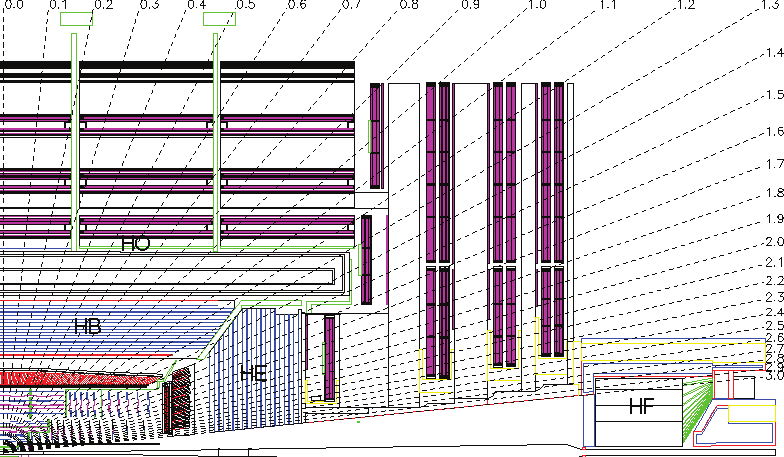
\includegraphics[width=0.95\textwidth]{\figpath/Chapter2/HCAL_subdet.pdf}
	\caption{A schematic of the CMS HCAL detector with its major subsystems labeled: HB, HE, HO, and HF.}
	\label{fig:CMS_HCAL}
\end{figure}

The HB occupies the region \absetalt{1.3} and contains alternating layers of brass and scintillator.
The number of nuclear interaction lengths ($\lambda_{0}$) ranges from 5.82 at $\eta=0$ to 10.6 at $\eta=1.3$.
Additionally the EB, which is directly in front of the HB, has 1.1$\lambda_{0}$ and can measure a portion of early developing hadronic showers, though not as accurately.
The properties of the brass used can be found in table~\ref{tab:HCAL_brass_properties} while the layer thicknesses and materials can be found in table~\ref{tab:HCAL_brass_thickness}.
Most of the plastic scintillating layers are 3.7\unit{mm} thick, but layer 16 is 9\unit{mm} thick so that is can sample more from late developing showers.
There is also an additional 9\unit{mm} thick layer 0 before the first absorbing layer so catch the showers which are initiated in the dead material between the EB and HB.
The scintillating tiles are arranged in a projective geometry (pointing close to the nominal interaction point) with the tiles occupying \mytimes{0.087}{0.087} in $\eta-\varphi$.
For \absetalt{1.479}, the HCAL cells map on to $5\times5$ arrays of ECAL crystals to form calorimeter towers.
Within each tower, the energy deposits in ECAL and HCAL cells are summed to define the calorimeter tower energies, subsequently used to provide the energies and directions of hadronic jets.
The scintillator is separated into 16 $\eta$ section and 36 $\varphi$ sections with almost 70000 tiles used.
The light is collected by wavelength shifting (WLS) fibers that encircle the tiles.
Fibers from several layers are read out by one hybrid photodiode (HPD), which are used for their large dynamic range and low sensitivity to magnetic fields.

\begin{table}[htbp]
\caption{Properties of the brass absorber used for the CMS HB.}
\centering
\begin{tabular}{|l|c|}%
\hline %
Property & Value \\%
\hline
Materials & Brass (70\% Copper and 30\% Zinc) or Steel \\%
Density & 8.53\unit{g/cm$^{\text{3}}$}\% \\%
Radiation Length & 1.49\unit{cm} \\%
Nuclear Interaction Length & 16.42\unit{cm}\\
\hline
\end{tabular}
\label{tab:HCAL_brass_properties}
\end{table}

\begin{table}[htbp]
\caption{Absorbing layer thicknesses and materials for the CMS HB}
\centering
\begin{tabular}{|l|c|c|}%
\hline %
Layer number(s) & Material & Thickness (\unit{mm}) \\%
\hline
1 & Steel & 40 \\%
2-9 & Brass & 50.5 \\%
10-15 & Brass & 56.5 \\%
16 & Steel & 75 \\%
\hline
\end{tabular}
\label{tab:HCAL_brass_thickness}
\end{table}

In the central region of the detector there are too few $\lambda_{0}$ to fully contain a hadronic shower.
For this reason the HO system was added as a scintillating tile extension to the HB.
The HO consists of five rings, each with a width of 2.536\unit{m} in the $z$-direction.
The most central ring, Ring 0, has two scintillating layers, one inside the solenoid and one outside the solenoid.
The other rings have only one layer outside of the solenoid, which acts as a 19.5\unit{cm} iron absorber layer.
This addition to the HB brings the total depth of the CMS calorimeter systems to 11.8$\lambda_{0}$.

The HE, a 17 layer sampling calorimeter, covers the \abseta{1.3}{3.0} region.
It consists of 79\unit{mm} brass absorbing layers and uses the same scintillating material as is used in the HB, but contains only 20916 tiles.
Within \absetalt{1.6} the granularity of these tiles is the same as for the HB, but at higher $\eta$ the approximate granularity becomes \mytimes{0.174}{0.174} in $\eta-\varphi$.
Like the HB, the HE also has a layer 0.
However, unlike the HB, the scintillating layers in the HE are grouped into ``depths'' before the light reaches the HPDs.
Fig~\ref{fig:CMS_HCAL_depth} shows a schematic of the CMS HCAL system where the different colors corresponds to the various depths.
This depth segmentation allows fore more precise recalibration of the HE, which receives a higher radiation dose than the HB.
When combined with the EE, this section of the detector corresponds to a length of 10$\lambda_{0}$.

\begin{figure}[!hbt]
	\centering
	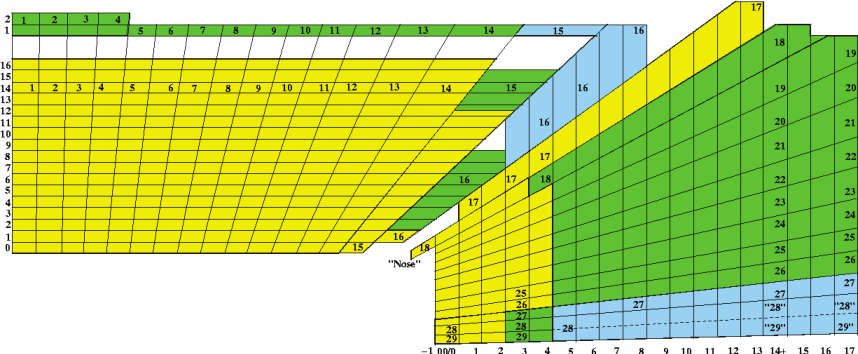
\includegraphics[width=0.95\textwidth]{\figpath/Chapter2/HCAL_tower_segmentation.pdf}
	\caption{A schematic of the HB and HE depth segmentation.}
	\label{fig:CMS_HCAL_depth}
\end{figure}

The HF uses steel as an absorber and embedded quartz fibers as the sensitive material.
The reason for the change in technology is that the HF needs to be able to withstand at least 100\unit{Mrad/year}.
The two halves of the HF are located 11.2\unit{m} from the interaction region, one on each end, and together they provide coverage in the range $3.0<\abs{\eta}<5.2$.
Unlike the other hadronic calorimeter systems, the HF does not have a piece of the ECAL in front of it.
Each HF calorimeter consist of 432 readout towers, containing almost 1000\unit{km} of 800\mum diameter long and short quartz fibers running parallel to the beam with a granularity of \mytimes{0.175}{0.175} in $\eta-\varphi$.
The long fibers run the entire depth of the HF calorimeter (165\unit{cm}, or approximately 10 interaction length), while the short fibers start at a depth of 22\unit{cm} from the front of the detector.
By reading out the two sets of fibers separately, it is possible to distinguish EM showers generated by electrons and photons, which deposit a large fraction of their energy in the long-fiber calorimeter segment, from those generated by hadrons, which produce on average nearly equal signals in both calorimeter segments.
The fibers make use of Cherenkov light read out by photomultiplier tubes (PMTs), which receive approximately 1 photoelectron for every 4\gev of deposited energy.

\subsection{Solenoid}

The central feature of the CMS apparatus is a superconducting solenoid of 6\unit{m} internal diameter, providing a magnetic field of 3.8\unit{T}.
The solenoid thus surrounds both the barrel and endcap parts of the silicon pixel and strip tracker, the ECAL, and the HCAL.
The high magnetic field allows CMS to have a relatively small size while also having sufficiently high bending of the high energy charged particles to measure their momenta in the tracker.

The magnet itself is made up of a 4-layer winding of reinforced NbTi superconductor cooled to 4.5\unit{K}.
Like the rest of CMS, this system needed to be modular and is constructed of 5 rings of equal length.
The cold mass of the magnet is 220 tonnes and it stores 2.35\unit{GJ} when the current is fully on.
Fig.~\ref{fig:CMS_solenoid} shows an artist's rendering of the solenoid.

\begin{figure}[!hbt]
	\centering
	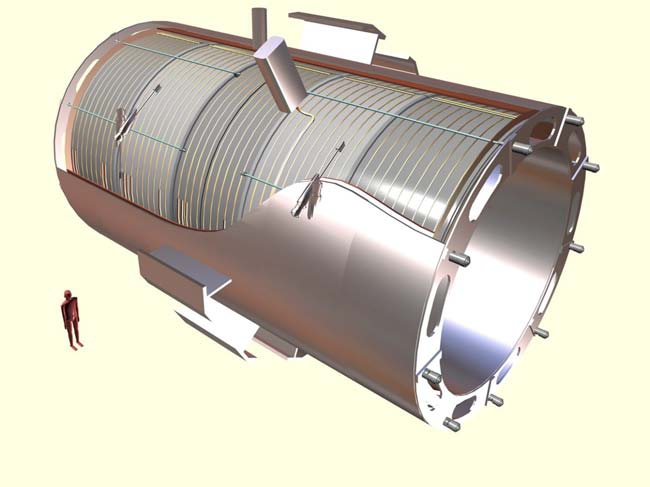
\includegraphics[width=0.95\textwidth]{\figpath/Chapter2/CMS_solenoid.jpg}
	\caption{An artists rendering of the CMS solenoid. The five superconducting rings can be seen inside the cryostat and support structure. A human figure is shown for comparison.}
	\label{fig:CMS_solenoid}
\end{figure}

\subsection{Muon System}

Muons are measured in gas-ionization detectors embedded in the steel flux-return yoke outside the solenoid in the pseudorapidity range \absetalt{2.4}, with detection planes made using three technologies: drift tubes (DTs), cathode strip chambers (CSCs), and resistive plate chambers (RPCs).
The barrel region of the detector contains DTs and RPCs, while the endcap region contains CSCs and RPCs.
The layout of the muon system can be seen in fig.~\ref{fig:CMS_muon_system}.
The iron yoke not only returns the flux from the solenoid, but also shields the muon chambers from stray hadrons.
The entire muon detection system has nearly 1 million electronic channels and weights in excess of 10000 tons.
The muon system on its own has a resolution of 15--40\% depending on $\abs{\eta}$.
Matching muons to tracks measured in the silicon tracker results in a relative transverse momentum resolution for muons with \ptrange{20}{100}\GeV of 1.3--2.0\% in the barrel and better than 6\% in the endcaps. The $p_{T}$ resolution in the barrel is better than 10\% for muons with \pt up to 1\TeV~\cite{Chatrchyan:2012xi}.

\begin{figure}[!hbt]
	\centering
	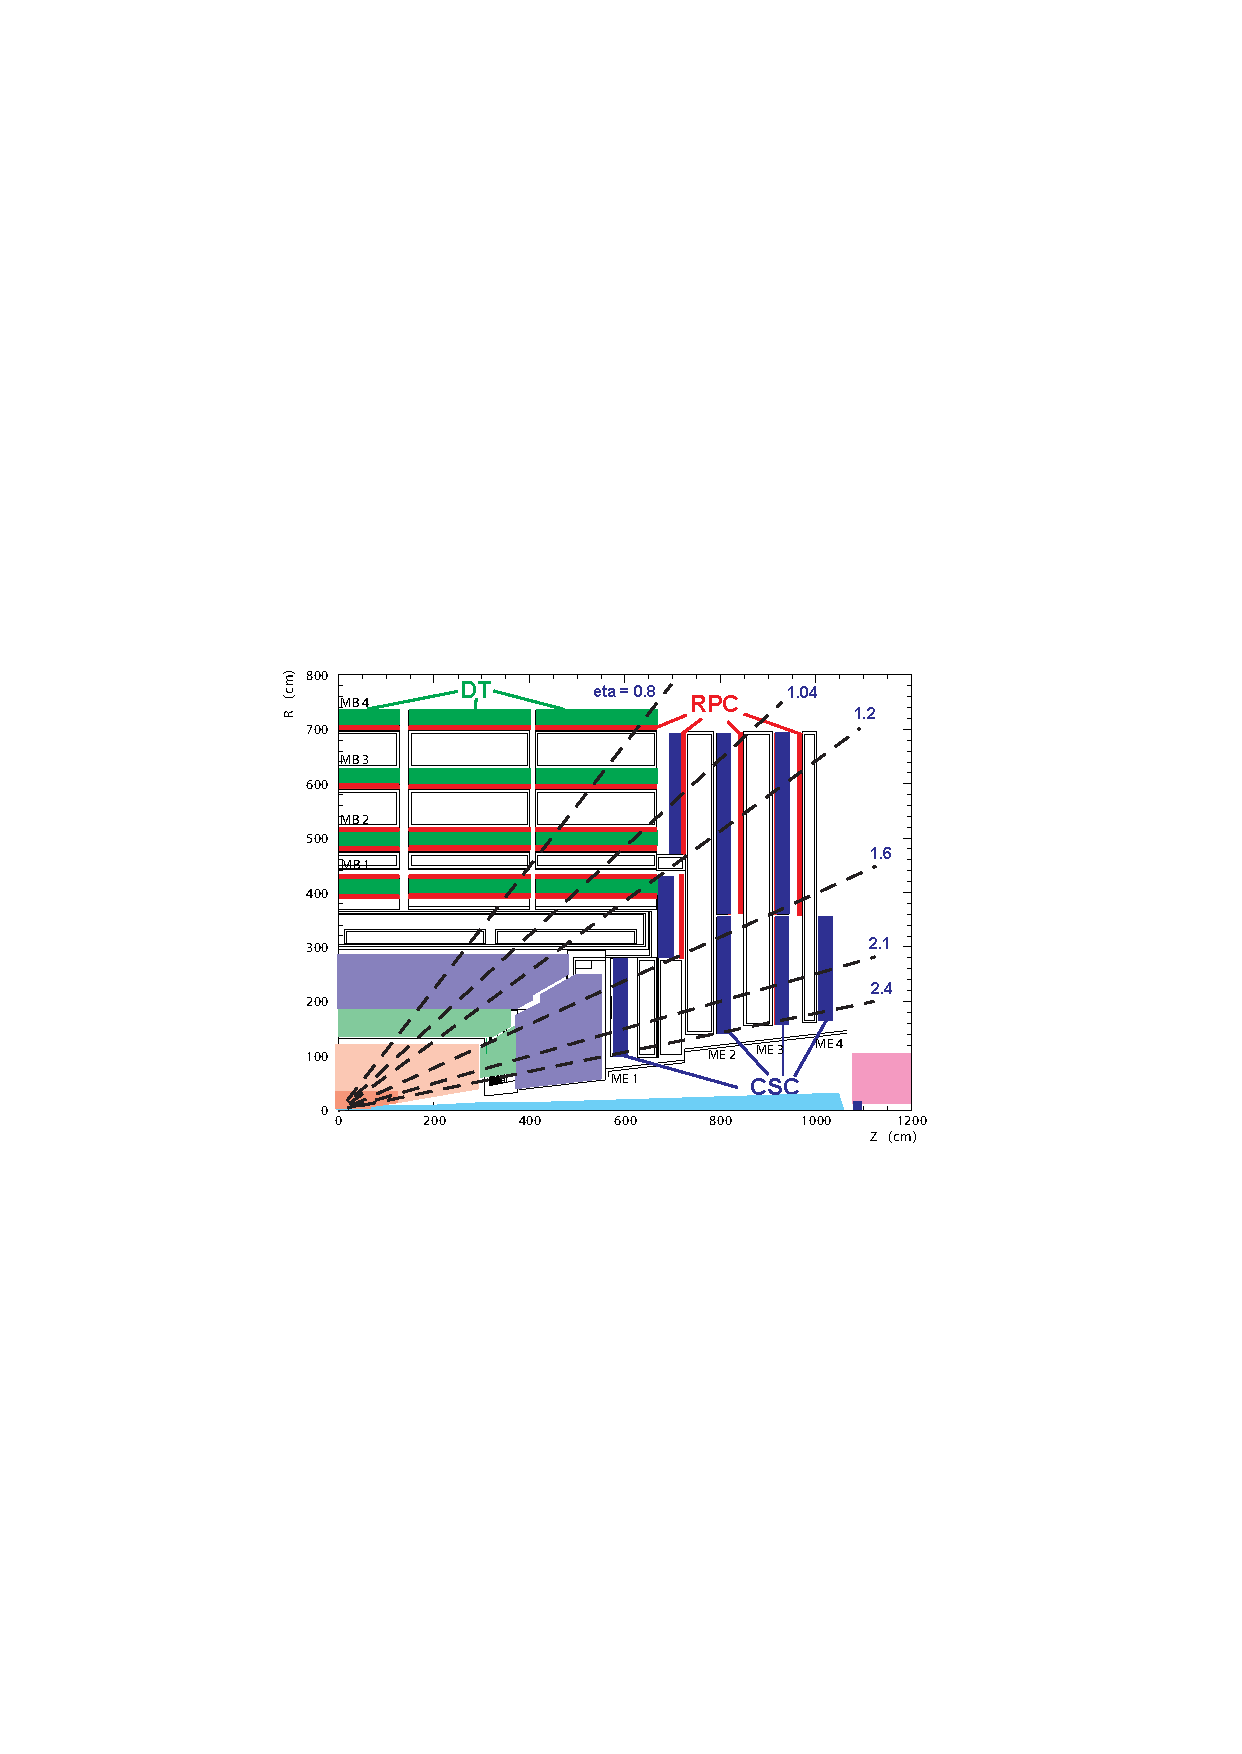
\includegraphics[width=0.95\textwidth]{\figpath/Chapter2/CMS_muon_system.pdf}
	\caption{Layout of the muon system with the three different detector technologies labeled.}
	\label{fig:CMS_muon_system}
\end{figure}

The DTs are divided into four stations named MB1 through MB4 (Muon Barrel), starting radially from the center of the detector outward.
The first three stations contain 12 chambers divided into three groups of four.
Two of the groups measure the $r-\varphi$ coordinates of the muon while the third group measures the $z$ coordinate.
However, MB4 does not have a group of chambers which measured the $z$ coordinate.
The four stations contain 250 DTs in total with a collective 172000 sensitive wires, covering an $\eta$ range of \absetalt{1.2}.
The chambers themselves contain a gas mixture of 85\% Ar and 15\% CO\textsubscript{2} and have gold-plated, stainless steel anode wires with a diameter of 50\mum.
Within \absetalt{0.8}, the MB stations can reconstruct a high-\pt muon track with an efficiency greater than 95\%.
The global $r-\varphi$ resolution is 100\mum.
Fig~\ref{fig:CMS_muon_system_DT} gives a transverse view of the DTs in one of the five wheels of CMS.

\begin{figure}[!hbt]
	\centering
	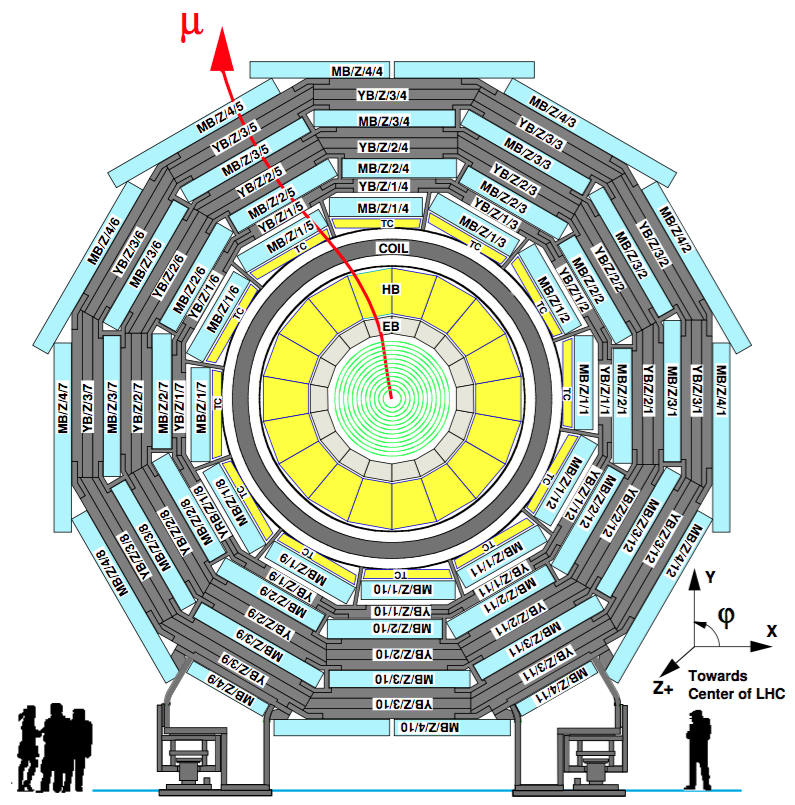
\includegraphics[width=0.95\textwidth]{\figpath/Chapter2/CMS_muon_system_DT}
	\caption{Transverse view of one of the five wheels of the CMS detector. The DTs and their layout can be clearly seen~\cite{Chatrchyan:2008aa}.}
	\label{fig:CMS_muon_system_DT}
\end{figure}

The CSCs are separated into four stations as well, names ME1 through ME4 (Muon Endcap), and cover \abseta{0.9}{2.4}.
ME1 has three groups of 72 CSC, ME2 and ME3 each have one group of 36 CSCs and one group of 72 CSCs, and ME4 has one group of 36 CSCs.
Thus each endcap contains 468 CSCs total.
Within a CSC the cathode strips are arranged radially in order to measure the $r-\varphi$ coordinate of the muon.
The anode wires are then arranged perpendicular to the strips in order to measure the $\eta$ coordinate.
The cathode strips themselves are made of a fiberglass and epoxy material called FR4, which is coated with 36\mum of copper.
The anode wires are gold-plated tungsten with a diameter of 50\mum (the first group of ME1 uses 30\mum wires).
There are approximately 220000 cathode strip readout channels and 180000 anode wire readout channels in total.
Each CSC contains a gas mixture of 40\% Ar, 50\% CO\textsubscript{2}, and 10\% CF\textsubscript{4}.

The RPCs are meant to aid in triggering on muons.
They cover out to \absetalt{1.6} and can provide information to the trigger system much faster than the DTs or CSCs.
The time resolution for the RPCs is less than 3\unit{ns}, whereas the DTs and CSCs have a maximum drift time of 400\unit{ns} 60\unit{ns}, respectively.
With such a small time resolution, the RPCs can precisely identify the bunch crossing time of a muon candidate.
MB1 and MB2 have one internal and one external group of RPCs, relative to the DTs.
MB3 and MB4 each have two internal groups of RPCs.
This amounts to 480 RPCs for the barrel.
The endcap has 3 stations of RPCs, 144 chambers in total, arranged in concentric circle on the iron return yoke.
The RPCs are a type of parallel plate detector with a gas mixture of 96.2\% C\textsubscript{2}H\textsubscript{2}F\textsubscript{4}, 3.5\% C\textsubscript{4}H\textsubscript{10}, and 0.3\% SF\textsubscript{6}.

\subsection{Trigger}

In order to provide as many collisions as possible to the experiments, the LHC must operate at a high luminosity (see sec.~\ref{sec:LHC}).
At the proposed LHC center-of-mass energies the p-p collision cross section is about 100\unit{mb}.
This, combined with the luminosity, gives us a collision rate of approximately 1\unit{MHz}.
At this rate it would be impossible for the experiment to store and process all of the raw information coming from the detector.
Thus a trigger system is implemented to reduce this rate and keep only the most interesting, and hopefully relevant, events.
%Keeping events most likely to contain new physics
CMS has implemented a two-tiered trigger system~\cite{Khachatryan:2016bia}.
The first level (L1), composed of custom hardware processors, uses information from the calorimeters and muon detectors to select events at a rate of around 100\unit{kHz} within a time interval of less than 4\mus.
The second level, known as the high-level trigger (HLT), consists of a farm of processors running a version of the full event reconstruction software optimized for fast processing, and reduces the event rate to less than 1\unit{kHz} before data storage.

\begin{figure}[!hbt]
	\centering
	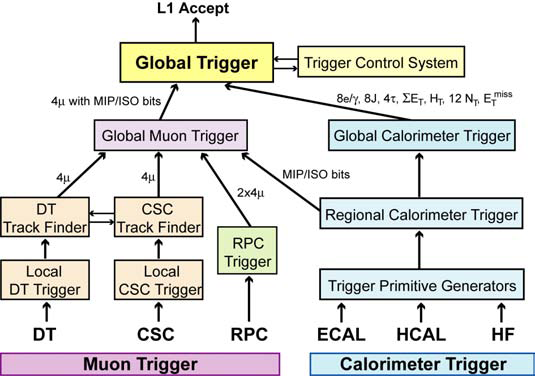
\includegraphics[width=0.95\textwidth]{\figpath/Chapter2/L1_architecture.png}
	\caption{The architecture of the L1 trigger system.}
	\label{fig:CMS_L1_architecture}
\end{figure}

The L1 trigger is is composed of custom built, programmable electronics including field programmable gate arrays (FPGAs), memory lookup tables (LUTs) and application specific integrated circuits (ASICs).
The components of this trigger system are arranged so that there can be local, regional, and global decision making (see fig.~\ref{fig:CMS_L1_architecture}).
Most of the sub-detectors send information to this trigger system, but due to the algorithmic complexity of track finding, the process would take too long if the tracker was included in the decision making process.
A new ``track trigger'' system is in the process of being developed, which would allow tracking information to be included in the L1 trigger decision making process.

The calorimeter side of the L1 trigger system starts with the Trigger Primitive Generators (TPG), which are constructed from energy deposits in the ECAL, HCAL, and HF.
These are then combined in the Regional Calorimeter Trigger (RCT), which groups the calorimeter towers into regions.
A region is defined as four towers for the barrel and endcap and one tower for the HF.
The regions are used to find photon and electron candidates, measure transverse energy sums ($\Sigma\ET$), and determine tau-jet vetoes.
The RCT also sends information to the Global Muon Trigger (GMT) about energy deposits to help determine if a muon candidate is isolated.
The information is then sent to the Global Calorimeter Trigger (GCT), which determines the jet candidates, providing up to four jets and four tau-jets from the central HCAL and four jets from the HF.
The GCT also calculates the \ET, \ETslash, and \HT, which is calculated as $\Sigma\ET$ for all jets above a certain threshold.

Each of the muon sub-detector's technologies (DT, CSC, and RPC) has a local trigger system.
The Regional Muon Trigger (RMT) takes the local trigger information from the DT and CSC and makes tracks using the DT and CSC Track Finders (DTTF and CSCTF).
In contrast, the RPCs are a form of dedicated trigger due to their small time resolution.
The Global Muon Trigger (GMT) combines the information from the RMT and RPCs to produce up to four muon candidates in each of the barrel and endcap regions.
The GMT also contains information about the \pt, charge, $\eta$, $\varphi$, quality, MIP, and isolation of each of the muon candidates.

Finally, the Global Trigger (GT) combines the GCT and GMT information to decide whether or not to store the event; a decision which is called a Level-1 Accept (L1A).
The GT also makes use of information about the sub-detector readouts and DAQ systems from the Trigger Control System (TCS). The L1A is returned to the sub-detectors by the Timing, Trigger, and Control (TTC) system.
This entire process takes 3.2\mus, an equivalent of $\mathcal{O}(100)$ bunch crossings, which means that the data must be pipelined in order to synchronize the steps in the trigger system.
Meanwhile, the high resolution data used for offline analysis is stored in memory. In 2012, the L1 Trigger rate was as high as 100\unit{kHz} with a dead time of only 3\%~\cite{Brooke:2013hnf}.

After the L1A decision, the High Level Trigger (HLT), a farm of more than 13000 central processing units (CPUs), further analyzes the events. The HLT 
system uses a form of the full offline reconstruction algorithms described in chapter~\ref{ch:event_reconstruction}, but also includes several optimizations to make the process faster. This is needed because, in contrast to offline processing, the HLT is limited by the number of events that can be stored in the pipeline. These optimizations include making the fasted algorithm run first, skipping a trigger path after the first failing quality filter, and considering smaller regions of the detector based on the L1 candidates. The menu of triggers to be run changes as the LHC and Monte Carlo (MC) simulation conditions change, even while CMS is operational. In 2012, the HLT had an output rate of 100\unit{kHz} and took 200\unit{ms} per event, $\mathcal{O}(100)$ times faster than the offline reconstruction~\cite{Trocino:2014jya}. Events that pass the HLT are then sorted into primary datasets (PDs) according to the passed triggers with as little overlap as possible.

\subsection{Luminosity Measurement}

Besides measuring the kinematics of each of the particles traversing the detector, CMS must also measure the instantaneous luminosity delivered by the LHC.
Both the pixel detector (section~\ref{sec:tracker_and_pixel}) and the HF (section~\ref{sec:hadron_calorimeter}) are able to measure the luminosity to varying degrees of accuracy.

The pixel detector has a very small granularity, which means that any given pixel is activated by at most one track per bunch crossing.
We can then create cluster by grouping nearby activated pixels, with the typical cluster containing an average of 5 pixels.
A minimum bias event typically creates 200 clusters~\cite{CMS-PAS-LUM-12-001}.
Even for events with 100 pileup (PU) interactions, a number significantly higher than was reached in 2012, the total pixel detector occupancy could be as low as 0.1\%.
This means that the number of pixel hits should scale linearly with the number of interactions per bunch crossing, which is shown in equation~\ref{eq:pixel_luminosity_measurement}~\cite{CMS-PAS-LUM-13-001}.

\begin{equation}
\mathcal{L}=\frac{\nu\average{n}}{\sigma_{vis}}
\label{eq:pixel_luminosity_measurement}
\end{equation}

Here the luminosity, $\mathcal{L}$, is proportional to average number of pixel clusters, \average{n}.
The other parameters are the LHC revolution frequency, $\nu=11246\unit{Hz}$ and the visible cross section, $\sigma_\text{vis}$, as calibrated by a Van der Meer scan~\cite{Balagura:2011yw}.
In 2012 this technique was used to measure the total integrated luminosity with a systematic uncertainty of 2.6\%.

Another method to measure the luminosity makes use of the HF, but due to some sever limitations in its accuracy, this measurement is only used as a cross-check for the pixel counting method.
What makes the HF suitable for this type of measurement is that it can safely be run during unstable beams~\cite{CMS-PAS-LUM-13-001}.
The average transverse energy per tower can be directly related to the luminosity or the average fraction of empty towers can be related to the mean number of interactions per crossing, which is more of in indirect measurement.
The benefit of using the HF is that it can make an online determination of the luminosity within 1\unit{s} to an accuracy of 1\%.
One downside is that even in 2012 the levels of pileup made the luminosity relationship non-linear.
Additionally, the calibration of this measurement can change due to drifts in the gains of the HF PMTs~\cite{Pedro2014}.